\subsection{Ballistic Reentry}\label{sec:example-ballistic-reentry}

One of the simplest problems for TAOS is a ballistic reentry. Ballistic flight occurs
when all of the control variables (angle of attack, angle of sideslip, bank angle, and
power setting) are zero so no guidance rules are required. If the vehicle's
configuration is assumed to remain the same throughout reentry, its trajectory can
be modeled with one segment that starts from the entry point and continues to
impact.

\taossubhead{Table File}

The only forces acting on the vehicle are from aerodynamic drag and gravity so only
a drag table is required. For conceptual design drag is often assumed to be only a
function of Mach number because altitude effects are usually small. The following
simple table file contains the axial-force coefficient as a function of Mach number:

\lstinputlisting[style=taosmanual]{examples/chapter04/ballistic-reentry-source.tbl.txt}

\taossubhead{Problem File}

The following problem file is used to calculate a set of ballistic reentry trajectories:

\lstinputlisting[style=taosmanual,basicstyle=\ttfamily\scriptsize]{examples/chapter04/ballistic-reentry-source.prb.txt}

Like all problems, it begins with a name enclosed in parentheses. This is followed by
data blocks that provide a title, an atmosphere model, and an earth model.

This problem involves only one vehicle so a single trajectory has been defined that
starts with segment number 1. The trajectory definition extends from the
\problemblock{*trajectory} keyword to the first \problemblock{*survey} keyword.
Data blocks within the trajectory definition have been indented to show the problem
structure.

\taossubhead{Trajectory Definition and Surveys}

Trajectories require initial conditions and at least one segment definition. Since this
problem has only one trajectory, specific initial conditions must be given. It cannot
be initialized from another trajectory because no other trajectories exist.

This set of trajectories is generic in that the location of the trajectory on the earth's
surface and the direction of the trajectories is not important. Thus, the initial latitude
and longitude can be set to zero and an initial heading angle of \ang{90} (east) can be
chosen. This is typical of trajectories calculated during conceptual design.

Two of the initial conditions, velocity and flight-path angle, are set to survey
variables. The \problemblock{*survey} data blocks near the end of the problem
provide values for these variables. Survey number 1, which varies the initial
flight-path angle, is the inner loop and has a set of specific values. Survey number 2,
which varies the initial velocity, is the outer loop. Its values have been given in the
``\texttt{lo}, \texttt{hi}, \texttt{inc}'' form so initial velocity takes on the values
15,000, 16,000, 17,000, and \SI{18000}{\foot\per\second}.

In general, trajectories must have a \problemblock{*print} data block giving a list of
variables that will be written to the printout file. Often this is the same list of
variables written to the EGS database file.

This trajectory only requires one segment. The \problemblock{*integ} data block is
used to enter an integration step size and a print interval, and an
\problemblock{*aero} data block is used to provide the name of the drag table. The
segment final condition ends the trajectory when the altitude becomes less than
zero.

Summary variables have been defined for the maximum dynamic pressure,
\statevar{max_q}, and the maximum axial $g$ loading, \statevar{max_g}. Even
though there is only one trajectory, trajectory numbers are still required in the
summary-variable definitions. In this case, the trajectory numbers are given as
subscripts enclosed in brackets. The vehicle is decelerating, giving negative axial
$g$'s, so the \texttt{min} function is used to select the most negative value and then
the \texttt{neg} operation is used to convert this to a positive number.

The \problemblock{*egs} data block is used to create an EGS database file so the
trajectory information can be plotted. The names given in the
\problemblock{*survey} data block, \statevar{gentry} and \statevar{ventry}, appear
in the EGS database file and are used for plotting.

\taossubhead{Results}

This problem calculates 16 trajectories, one for each combination of survey values.
On a Silicon Graphics workstation, the problem runs in about 9 seconds so it takes
a little over 0.5 seconds to compute each trajectory.

The following listing is typical of the trajectory printout for this problem:

\begin{center}
\begin{minipage}{0.98\linewidth}
\lstinputlisting[style=taosmanual,basicstyle=\ttfamily\tiny]{examples/chapter04/ballistic-reentry-printout.txt}
\end{minipage}
\end{center}

This page corresponds to the first trajectory computed by TAOS, which is for an
initial velocity of \SI{15000}{\foot\per\second} and an initial flight-path angle of
\ang{-35}.

The summary variables are tabulated as a function of the survey variables on the last
printout page as follows:

\begin{center}
\begin{minipage}{0.86\linewidth}
\lstinputlisting[style=taosmanual,basicstyle=\ttfamily\scriptsize]{examples/chapter04/ballistic-reentry-summary.txt}
\end{minipage}
\end{center}

The trajectory data is plotted with EGS in
\cref{fig:example-reentry-altitude-range,fig:example-reentry-velocity-time,fig:example-reentry-max-q,fig:example-reentry-max-g}.
The first two figures show four trajectories for different initial flight-path angles and
a constant initial velocity. The last two figures show the summary variables plotted
as a function of the survey variables.

\begin{figure}[htbp]
  \centering
  \resizebox{0.84\linewidth}{!}{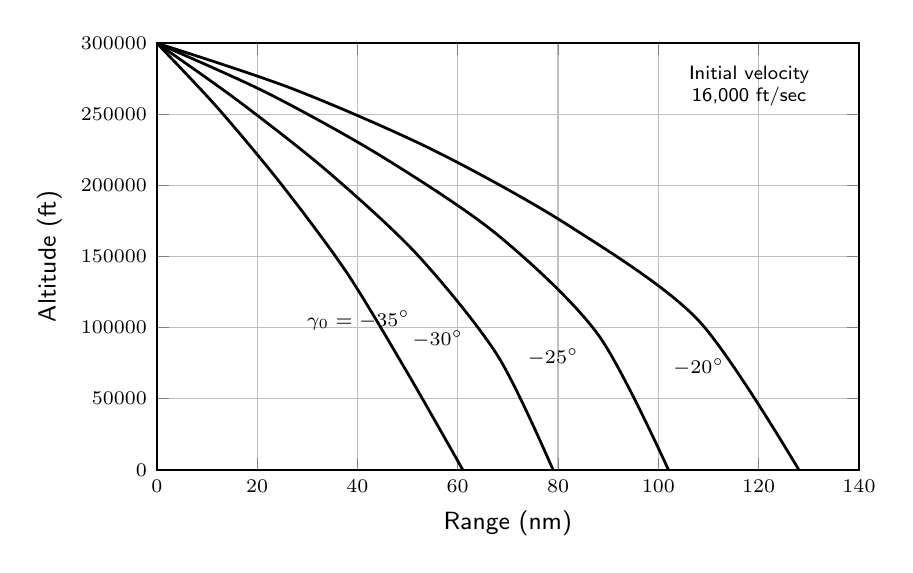
\begin{tikzpicture}
\begin{axis}[
  width=10.5cm,height=7.0cm,
  xmin=0,xmax=140,ymin=0,ymax=300000,
  xtick={0,20,40,60,80,100,120,140},
  ytick={0,50000,100000,150000,200000,250000,300000},
  grid=major,
  axis line style={line width=0.8pt},
  tick label style={font=\scriptsize},
  label style={font=\sffamily\small},
  xlabel={Range (nm)},ylabel={Altitude (ft)},
  scaled y ticks=false,
  yticklabel style={/pgf/number format/fixed,/pgf/number format/1000 sep={}},
]
  \addplot[line width=1.0pt,smooth] coordinates {(0,300000) (12,255000) (25,200000) (38,138000) (50,68000) (61,0)};
  \addplot[line width=1.0pt,smooth] coordinates {(0,300000) (16,260000) (34,210000) (52,151000) (68,80000) (79,0)};
  \addplot[line width=1.0pt,smooth] coordinates {(0,300000) (22,265000) (45,220000) (68,165000) (88,95000) (102,0)};
  \addplot[line width=1.0pt,smooth] coordinates {(0,300000) (27,268000) (55,225000) (82,172000) (108,105000) (128,0)};
  \node[font=\sffamily\scriptsize,anchor=west] at (axis cs:28,105000) {$\gamma_0=-35^\circ$};
  \node[font=\sffamily\scriptsize,anchor=west] at (axis cs:49,92000) {$-30^\circ$};
  \node[font=\sffamily\scriptsize,anchor=west] at (axis cs:72,79000) {$-25^\circ$};
  \node[font=\sffamily\scriptsize,anchor=west] at (axis cs:101,72000) {$-20^\circ$};
  \node[font=\sffamily\scriptsize,align=center,anchor=east] at (axis cs:132,270000) {Initial velocity\\16,000 ft/sec};
\end{axis}
\end{tikzpicture}
}
  \caption{Altitude versus range for example ballistic trajectories.}
  \label{fig:example-reentry-altitude-range}
\end{figure}

\begin{figure}[htbp]
  \centering
  \resizebox{0.84\linewidth}{!}{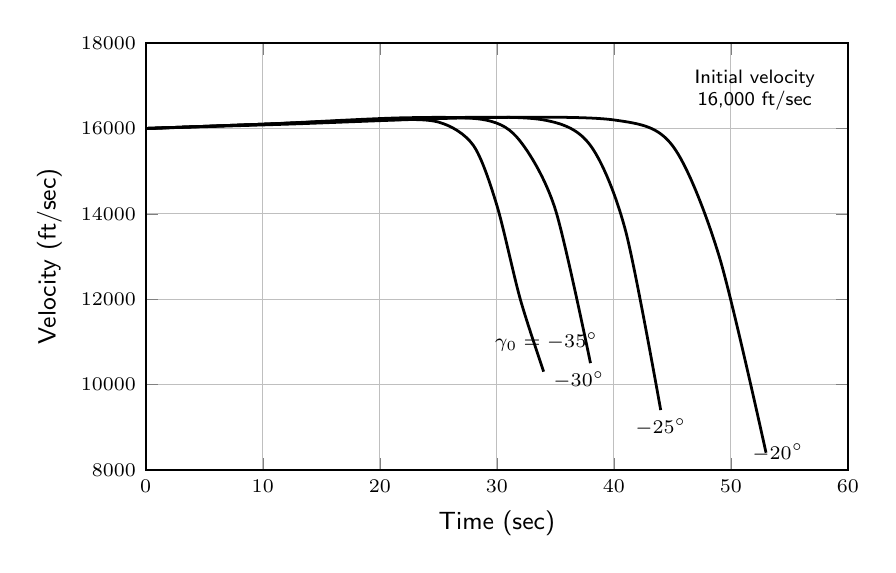
\begin{tikzpicture}
\begin{axis}[
  width=10.5cm,height=7.0cm,
  xmin=0,xmax=60,ymin=8000,ymax=18000,
  xtick={0,10,20,30,40,50,60},
  ytick={8000,10000,12000,14000,16000,18000},
  grid=major,
  axis line style={line width=0.8pt},
  tick label style={font=\scriptsize},
  label style={font=\sffamily\small},
  xlabel={Time (sec)},ylabel={Velocity (ft/sec)},
  scaled y ticks=false,
  yticklabel style={/pgf/number format/fixed,/pgf/number format/1000 sep={}},
]
  \addplot[line width=1.0pt,smooth] coordinates {(0,16000) (10,16100) (20,16200) (25,16150) (28,15600) (30,14200) (32,12000) (34,10300)};
  \addplot[line width=1.0pt,smooth] coordinates {(0,16000) (10,16100) (22,16250) (29,16200) (32,15700) (35,14100) (38,10500)};
  \addplot[line width=1.0pt,smooth] coordinates {(0,16000) (10,16100) (25,16250) (34,16200) (38,15600) (41,13600) (44,9400)};
  \addplot[line width=1.0pt,smooth] coordinates {(0,16000) (12,16100) (28,16250) (40,16200) (45,15600) (49,13000) (53,8400)};
  \node[font=\sffamily\scriptsize,anchor=west] at (axis cs:29,11000) {$\gamma_0=-35^\circ$};
  \node[font=\sffamily\scriptsize,anchor=west] at (axis cs:34,10100) {$-30^\circ$};
  \node[font=\sffamily\scriptsize,anchor=west] at (axis cs:41,9000) {$-25^\circ$};
  \node[font=\sffamily\scriptsize,anchor=west] at (axis cs:51,8400) {$-20^\circ$};
  \node[font=\sffamily\scriptsize,align=center,anchor=east] at (axis cs:58,16900) {Initial velocity\\16,000 ft/sec};
\end{axis}
\end{tikzpicture}
}
  \caption{Velocity versus time for example ballistic trajectories.}
  \label{fig:example-reentry-velocity-time}
\end{figure}

\begin{figure}[htbp]
  \centering
  \resizebox{0.84\linewidth}{!}{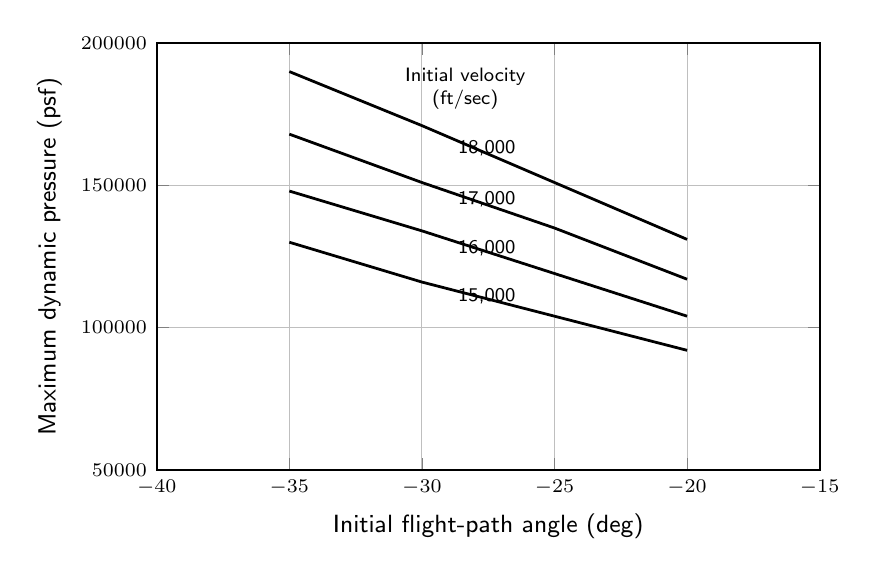
\begin{tikzpicture}
\begin{axis}[
  width=10.0cm,height=7.0cm,
  xmin=-40,xmax=-15,ymin=50000,ymax=200000,
  xtick={-40,-35,-30,-25,-20,-15},
  ytick={50000,100000,150000,200000},
  grid=major,
  axis line style={line width=0.8pt},
  tick label style={font=\scriptsize},
  label style={font=\sffamily\small},
  xlabel={Initial flight-path angle (deg)},
  ylabel={Maximum dynamic pressure (psf)},
  ylabel style={align=center},
  scaled y ticks=false,
  yticklabel style={/pgf/number format/fixed,/pgf/number format/1000 sep={}},
]
  \addplot[line width=1.0pt] coordinates {(-35,130000) (-30,116000) (-25,104000) (-20,92000)};
  \addplot[line width=1.0pt] coordinates {(-35,148000) (-30,134000) (-25,119000) (-20,104000)};
  \addplot[line width=1.0pt] coordinates {(-35,168000) (-30,151000) (-25,135000) (-20,117000)};
  \addplot[line width=1.0pt] coordinates {(-35,190000) (-30,171000) (-25,151000) (-20,131000)};
  \node[font=\sffamily\scriptsize,align=center,anchor=west] at (axis cs:-31,184000) {Initial velocity\\(ft/sec)};
  \node[font=\sffamily\scriptsize,anchor=west] at (axis cs:-29,163000) {18,000};
  \node[font=\sffamily\scriptsize,anchor=west] at (axis cs:-29,145000) {17,000};
  \node[font=\sffamily\scriptsize,anchor=west] at (axis cs:-29,128000) {16,000};
  \node[font=\sffamily\scriptsize,anchor=west] at (axis cs:-29,111000) {15,000};
\end{axis}
\end{tikzpicture}
}
  \caption{Maximum dynamic pressure for example ballistic trajectories.}
  \label{fig:example-reentry-max-q}
\end{figure}

\begin{figure}[htbp]
  \centering
  \resizebox{0.84\linewidth}{!}{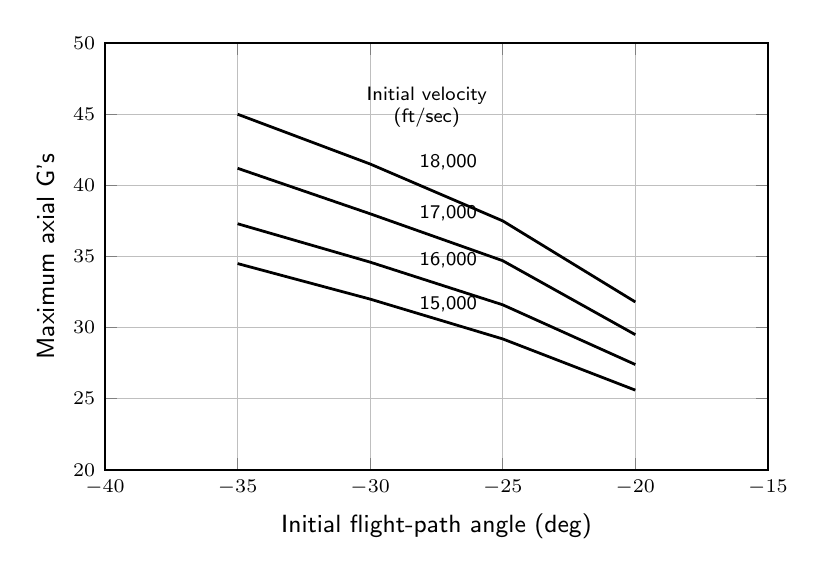
\begin{tikzpicture}
\begin{axis}[
  width=10.0cm,height=7.0cm,
  xmin=-40,xmax=-15,ymin=20,ymax=50,
  xtick={-40,-35,-30,-25,-20,-15},
  ytick={20,25,30,35,40,45,50},
  grid=major,
  axis line style={line width=0.8pt},
  tick label style={font=\scriptsize},
  label style={font=\sffamily\small},
  xlabel={Initial flight-path angle (deg)},
  ylabel={Maximum axial G's},
  ylabel style={align=center},
]
  \addplot[line width=1.0pt] coordinates {(-35,34.5) (-30,32.0) (-25,29.2) (-20,25.6)};
  \addplot[line width=1.0pt] coordinates {(-35,37.3) (-30,34.6) (-25,31.6) (-20,27.4)};
  \addplot[line width=1.0pt] coordinates {(-35,41.2) (-30,38.0) (-25,34.7) (-20,29.5)};
  \addplot[line width=1.0pt] coordinates {(-35,45.0) (-30,41.5) (-25,37.5) (-20,31.8)};
  \node[font=\sffamily\scriptsize,align=center,anchor=west] at (axis cs:-30.5,45.5) {Initial velocity\\(ft/sec)};
  \node[font=\sffamily\scriptsize,anchor=west] at (axis cs:-28.5,41.6) {18,000};
  \node[font=\sffamily\scriptsize,anchor=west] at (axis cs:-28.5,38.0) {17,000};
  \node[font=\sffamily\scriptsize,anchor=west] at (axis cs:-28.5,34.7) {16,000};
  \node[font=\sffamily\scriptsize,anchor=west] at (axis cs:-28.5,31.6) {15,000};
\end{axis}
\end{tikzpicture}
}
  \caption{Maximum axial G's for example ballistic trajectories.}
  \label{fig:example-reentry-max-g}
\end{figure}
